\documentclass[11pt]{article}

\usepackage{amsmath,amssymb,amsfonts}
\usepackage{graphicx}
\usepackage{pgfplots}
\usepackage{multicol}
\usepackage{enumitem}


\setlength{\topmargin}{-.5in} \setlength{\textheight}{9.25in}
\setlength{\oddsidemargin}{0in} \setlength{\textwidth}{6.8in}


\begin{document}

\Large

\noindent{\bf Name: \hfill Date: \hfill Quiz 3 \hfill Precalculus - Hargus}

\medskip\hrule
\vspace{10pt}

\begin{enumerate}

\item (20 points) Evaluate the expression.
\begin{multicols}{2}
\begin{enumerate}
    \item $\log_{3}{81}$ \\
    \item $\log_{4}{\frac{1}{\sqrt[3]{16}}}$ \\
\end{enumerate}
\end{multicols}

\item (10 points) Write the equation for an exponential function for a city which initially has 10 people and for which the population increases by $\%50$ every year.

$$f(x) = \rule{5cm}{0.15mm}$$

\item (15 points) Solve for $x$.
\begin{multicols}{2}
\begin{enumerate}[itemsep=25pt]
    \item $\log_{3}{x} = 2$
    \item $5^x = 15$
    \item $\log_{2}{x^2} = 2 $
\end{enumerate}
\end{multicols}

\item (15 points) The graph of $\ln(x)$ is shown below. Please draw the graph of $\ln(-x) + 1$.
\\

\vspace{10pt}
\begin{center}
\begin{tikzpicture}
\begin{axis}[ xlabel={$x$}, ylabel={$y$}
  ,axis lines=middle
  ,samples=1000, grid, thick
  ,domain=-10:10
  ,axis equal
  ,legend pos=outer north east
  ,xmin=-5, xmax=5,
  ,ymin=-5, ymax=5
  ]
\addplot+[no marks] {ln(x)};
\addlegendentry{$f(x)$}
\end{axis}
\end{tikzpicture}
\end{center}

\item (5 points) Extra credit: Solve $\ln(3x-2)+\ln(x-2)=2\ln(x)$ \textbf{algebraically}.

\end{enumerate}

\end{document} 